\section{Method}
\label{sec:method}

\subsection{System Model}

We consider $N$ autonomous agents (\emph{tenders}), each tending a
portion of a shared substrate. Agent $i$ has a parameter vector
$\mathbf{p}_i \in \mathbb{R}^{d_i}$ and an objective function $f_i$
toward an objective. The substrate couples the agents: agent
$i$'s objective reading depends not only on its own parameters but
also on other agents' parameters through hidden coupling channels:
\begin{equation}
  f_i(\mathbf{p}_i, \mathbf{p}_{j \neq i}) = g_i(\mathbf{p}_i) +
    \sum_{j \neq i} c_{ji}(\mathbf{p}_j)
\end{equation}
where $g_i$ is the agent's own response and $c_{ji}$ is the coupling
contribution from agent $j$ to agent $i$. The coupling function
$c_{ji}$ may be linear, nonlinear, or discontinuous. The coupling
structure---which agents affect which, through which channels, at
what strength---is unknown. Discovering it is the goal.

\subsection{Agent Operation}

Each agent runs a continuous trial loop. In normal operation, the
agent samples a parameter vector via a metaheuristic search
strategy (e.g., TPE, CMA-ES, NSGA-II), applies it to the substrate, reads back
its objective, and records the result. This is the \texttt{OPTIMIZE}
state---the agent's default behavior.

The coordination protocol interrupts this loop periodically to run
detection rounds. Crucially, the perturbations during detection
operate on the \emph{same parameters} the agent controls during
normal operation---the same knobs, within the same defined bounds.
Safety is actively enforced through guardrails: per-trial checks on
objective values and system state that reject configurations
exceeding safe operating limits. The IMPULSE\_CALIB phase probes at
decreasing scale and backs off immediately on any guardrail
violation. Only an amplitude that passes all guardrails is locked
for the push block.

The protocol does not inject faults, disrupt services, or push the
system outside its operating envelope. It adjusts known control
parameters to the edge of their range, observes the response, and
returns to neutral. The system continues operating throughout;
detection is non-destructive. This distinguishes the approach from
chaos engineering or fault injection, which deliberately break
components to test resilience.

\subsection{The Impulse Protocol}

\subsubsection{Sender State Machine}

A detection round for the sender consists of eight states:

\begin{enumerate}
  \item \textbf{\texttt{OPTIMIZE}}: Normal parameter exploration. After
    a minimum number of completed trials ($\geq 15$) and at least two
    active agents, the agent attempts to acquire the sender lease.

  \item \textbf{\texttt{HOLD\_CALIB}}: The sender establishes neutral
    hold parameters---values where its own objective is stable and the
    system is alive. When hold parameters are provided in
    configuration, this step is immediate. Otherwise, the sender
    searches for flat parameters by sampling its objective at
    candidate neutral values and accepting when the standard deviation
    falls below a threshold ($\sigma < 0.05$).

  \item \textbf{\texttt{IMPULSE\_CALIB}}: The sender probes at
    decreasing perturbation scale to find a safe amplitude. Starting
    at full scale ($1.0$), it drives its top-3 parameters (by range)
    toward their upper bounds. If guardrails are violated (e.g., the
    system destabilizes), it backs off: $1.0 \to 0.5 \to 0.25 \to
    0.125$. The first scale that passes becomes the locked amplitude
    for the entire push block. This adaptive calibration ensures the
    perturbation is large enough to produce a detectable signal but
    not so large as to harm the live system.

  \item \textbf{\texttt{PUSH}}: The sender perturbs at the locked
    scale for $B_{\text{push}}$ consecutive trials. Each trial applies
    the extreme parameters, reads back, and records the objective.
    The coupling signal propagates through the substrate to any
    coupled receivers.

  \item \textbf{\texttt{PAUSE}}: The sender returns to neutral hold
    parameters for $B_{\text{pause}}$ consecutive trials. This is the
    ABA recovery---the coupling signal should revert. The receiver's
    signal during this window serves as the post-intervention
    baseline.

  \item \textbf{\texttt{DONE}}: The sender releases the lease and
    clears coordination state.

  \item \textbf{\texttt{COOLDOWN}}: The sender waits a short period
    (5 trials) before re-acquiring, giving other agents a chance to
    take their turn. This enforces fairness in turn-taking.

  \item \textbf{\texttt{HOLD}} (receiver): While any sender holds the
    lease, all other agents enter HOLD---fixing their parameters at
    neutral values and acting as passive sensors. Each hold trial is
    tagged with the sender's current lease phase, so the detector
    can later segment receiver observations into push-window and
    pause-window samples.
\end{enumerate}

\subsubsection{Lease and Turn-Taking}

Only one agent may be sender at any time. A shared lease
(row in a coordination database) enforces this. The lease uses:

\begin{description}
  \item[Fencing tokens] A monotonically increasing token is written
    on each lease acquisition. Every lease mutation (heartbeat,
    budget decrement, release) is guarded by a \texttt{WHERE token =
    $t$} check. If another agent steals the lease (via stale
    recovery), the old sender's token no longer matches and its
    writes are silently rejected---preventing split-brain.
  \item[Count-based budget] The lease tracks
    \texttt{push\_remaining} and \texttt{pause\_remaining} counters
    rather than wall-clock expiry. The sender's turn lasts exactly
    as long as it has budget, avoiding premature expiry when trials
    run slowly (database retries, slow effectuation).
  \item[Heartbeat staleness] A crashed sender's lease is recovered
    when its heartbeat exceeds $5 \times$ the worst-case trial
    duration. Budget alone is insufficient because a crashed sender's
    counters stay positive forever.
\end{description}

\begin{figure*}[t]
\centering
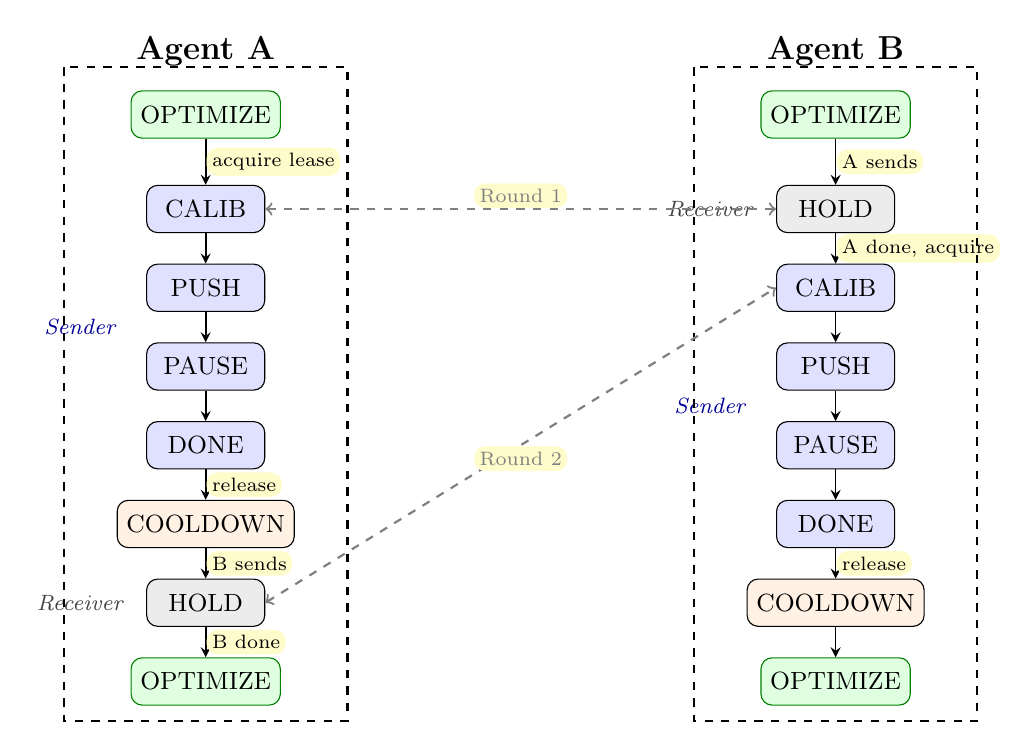
\begin{tikzpicture}[
  node distance=1.0cm,
  st/.style={rectangle, draw, rounded corners, minimum width=1.5cm, minimum height=0.6cm, font=\small},
  send/.style={st, fill=blue!12},
  recv/.style={st, fill=gray!15},
  shared/.style={st, fill=green!12, draw=green!50!black},
  cooldown/.style={st, fill=orange!10},
  arrow/.style={->, >=stealth, semithick},
  tlabel/.style={font=\scriptsize, fill=yellow!20, rounded corners, inner sep=2pt},
]

% ══ Column positions ══
\def\xa{0}
\def\xb{8}

% ══ Agent A (left) ══
\node[font=\large\bfseries] at (\xa, 1.0) {Agent A};

\node[shared] (aopt0) at (\xa, 0.2) {OPTIMIZE};
\node[send] (acalib) at (\xa, -1.0) {CALIB};
\node[send] (apush) at (\xa, -2.0) {PUSH};
\node[send] (apause) at (\xa, -3.0) {PAUSE};
\node[send] (adone) at (\xa, -4.0) {DONE};
\node[cooldown] (acool) at (\xa, -5.0) {COOLDOWN};
\node[recv] (ahold) at (\xa, -6.0) {HOLD};
\node[shared] (aopt1) at (\xa, -7.0) {OPTIMIZE};

\draw[arrow] (aopt0) -- node[tlabel, right] {acquire lease} (acalib);
\draw[arrow] (acalib) -- (apush);
\draw[arrow] (apush) -- (apause);
\draw[arrow] (apause) -- (adone);
\draw[arrow] (adone) -- node[tlabel, right] {release} (acool);
\draw[arrow] (acool) -- node[tlabel, right] {B sends} (ahold);
\draw[arrow] (ahold) -- node[tlabel, right] {B done} (aopt1);

% Sender/Receiver labels
\node[font=\footnotesize\itshape, blue!60!black] at (\xa-1.6, -2.5) {Sender};
\node[font=\footnotesize\itshape, gray!50!black] at (\xa-1.6, -6.0) {Receiver};

% Agent A box
\draw[dashed, thick] (\xa-1.8, 0.8) rectangle (\xa+1.8, -7.5);

% ══ Agent B (right) ══
\node[font=\large\bfseries] at (\xb, 1.0) {Agent B};

\node[shared] (bopt0) at (\xb, 0.2) {OPTIMIZE};
\node[recv] (bhold) at (\xb, -1.0) {HOLD};
\node[send] (bcalib) at (\xb, -2.0) {CALIB};
\node[send] (bpush) at (\xb, -3.0) {PUSH};
\node[send] (bpause) at (\xb, -4.0) {PAUSE};
\node[send] (bdone) at (\xb, -5.0) {DONE};
\node[cooldown] (bcool) at (\xb, -6.0) {COOLDOWN};
\node[shared] (bopt1) at (\xb, -7.0) {OPTIMIZE};

\draw[arrow] (bopt0) -- node[tlabel, right] {A sends} (bhold);
\draw[arrow] (bhold) -- node[tlabel, right] {A done, acquire} (bcalib);
\draw[arrow] (bcalib) -- (bpush);
\draw[arrow] (bpush) -- (bpause);
\draw[arrow] (bpause) -- (bdone);
\draw[arrow] (bdone) -- node[tlabel, right] {release} (bcool);
\draw[arrow] (bcool) -- (bopt1);

% Sender/Receiver labels
\node[font=\footnotesize\itshape, gray!50!black] at (\xb-1.6, -1.0) {Receiver};
\node[font=\footnotesize\itshape, blue!60!black] at (\xb-1.6, -3.5) {Sender};

% Agent B box (same size as A)
\draw[dashed, thick] (\xb-1.8, 0.8) rectangle (\xb+1.8, -7.5);

% ══ Lease coordination ══
% Round 1: A enters CALIB (holds lease), B observes and enters HOLD
\draw[dashed, gray, thick, <->] (acalib.east) -- node[tlabel, above] {Round 1} (bhold.west);

% Round 2: B enters CALIB (holds lease), A observes and enters HOLD
\draw[dashed, gray, thick, <->] (ahold.east) -- node[tlabel, below] {Round 2} (bcalib.west);

\end{tikzpicture}
\caption{Two-agent turn-taking in the impulse protocol. Both agents
start in OPTIMIZE. In Round 1, Agent A acquires the sender lease and
enters the detection cycle: CALIB (hold neutral, find safe perturbation
amplitude), PUSH (drive parameters to extremes), PAUSE (return to
neutral), DONE (release lease). Agent B observes the active lease
and enters HOLD as passive receiver throughout A's detection cycle.
After cooldown, the roles reverse for Round 2. CALIB encompasses
HOLD-CALIB (parameter flatness search) and IMPULSE-CALIB (adaptive
perturbation with guardrail backoff). Dashed arrows show lease
pairing: while one agent holds the sender lease, the partner is in
HOLD.}
\label{fig:state-machine}
\end{figure*}


\subsection{CFAR Step-Change Detection}

After rounds complete, the detector evaluates each ordered
sender--receiver pair. For each pair, the receiver's hold-trial
objectives are segmented by the sender's push/pause timestamps into:

\begin{itemize}
  \item \emph{Baseline window}: receiver values during the sender's
    pause phase (post-intervention recovery)
  \item \emph{Push window}: receiver values during the sender's push
    phase
\end{itemize}

A noise-adaptive threshold is computed from the baseline:
\begin{equation}
  T = k \cdot \widehat{\sigma}_{\text{baseline}}, \quad
  k = N_{\text{ref}} \left( P_{\text{fa}}^{-1/N_{\text{ref}}} - 1 \right)
  \label{eq:threshold}
\end{equation}
where $\widehat{\sigma}$ is the scaled median absolute deviation
(MAD $\times$ 1.4826, a robust $\sigma$-estimator), $N_{\text{ref}}$
is the number of baseline samples, and $P_{\text{fa}} = 0.05$.

A round is \emph{detected} if both:
\begin{align}
  |\text{push\_median} - \text{baseline\_median}| &\geq T \label{eq:rising} \\
  |\text{push\_median} - \text{pause\_median}| &\geq T \label{eq:falling}
\end{align}

Condition~(\ref{eq:rising}) detects the step; condition~(\ref{eq:falling})
enforces reversibility. A monotonic drift would satisfy
(\ref{eq:rising}) but fail (\ref{eq:falling}) because the pause-phase
values would not revert to baseline.

\subsection{Observation Parameters}
\label{sec:obs-params}

All experiments use the following parameters unless otherwise stated:

\begin{center}
\begin{tabular}{ll}
  \toprule
  Parameter & Value \\
  \midrule
  Push block size ($B_{\text{push}}$) & 15 trials \\
  Pause block size ($B_{\text{pause}}$) & 15 trials \\
  Min.\ exploration before detection & 15 trials \\
  Cooldown (turn-taking fairness) & 5 trials \\
  Impulse calibration scales & $1.0, 0.5, 0.25, 0.125$ \\
  Hold parameters & midpoint ($50, 50, 50$) \\
  Push target & top-3 params $\to$ upper bound \\
  CFAR $P_{\text{fa}}$ & 0.05 \\
  Min.\ reference cells (baseline) & 3 \\
  Min.\ test cells (push/pause) & 3 \\
  \bottomrule
\end{tabular}
\end{center}

Detection boundaries are parameterized by observation budget.
Increasing block sizes or the number of rounds lowers the boundary,
as the CFAR scale factor $k$ decreases with more reference cells.
The impulse calibration adapts perturbation amplitude to system
constraints---this parameter is not fixed but discovered per system.
